% 12 variables in here:
% H_1 = 10.0, H_2 = 10.0, H_3 = 10.0, U_1 = 0.0, U_2 = 0.0, U_3 = 0.0, h_1 = 10.0, h_2 = 10.0, h_3 = 10.0, u_1 = -1.0, u_2 = 0.0, u_3 = 0.0
\begin{figure}[h!]
\centering
  % \subfigure[] {
  %   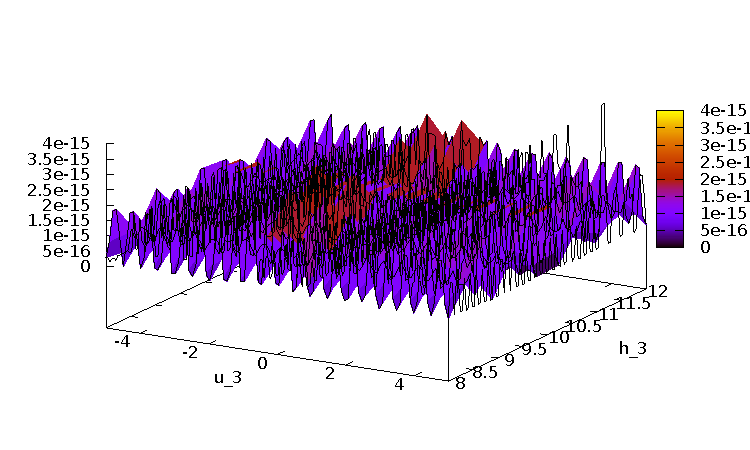
\includegraphics[scale=\zoomfactor]{{{equidist_3_alles_default_ausser_p1_10_-1/10.0_10.0_10.0_0.0_0.0_0.0_10.0_10.0_y_-1.0_0.0_xf00}}}
  % }
  \subfigure[Impulse error for $p_2^L$] {
    \begin{tikzpicture}
      \node at (0,0) {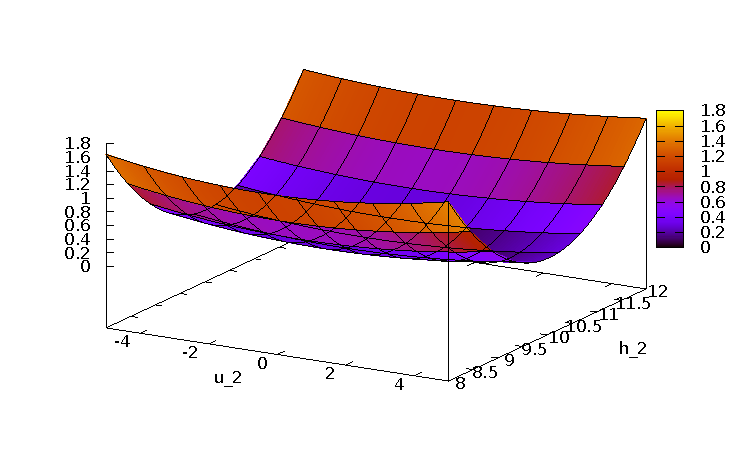
\includegraphics[scale=\zoomfactor]{{{equidist_3_alles_default_ausser_p1_10_-1/10.0_10.0_10.0_0.0_0.0_0.0_10.0_y_10.0_-1.0_x_0.0f01}}}};
      \node[align=right, text width=3cm] at (.2,1.33) {\textsf{\tiny{Impulse error}}};
      \draw(1.8,1.34) -- +(.4cm,0);
    \end{tikzpicture}
  }
  \subfigure[Impulse error for $p_3^L$] {
    \begin{tikzpicture}
      \node at (0,0) {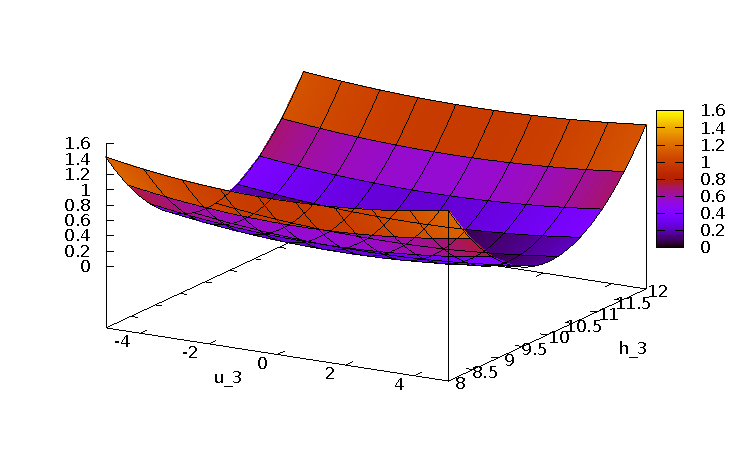
\includegraphics[scale=\zoomfactor]{{{equidist_3_alles_default_ausser_p1_10_-1/10.0_10.0_10.0_0.0_0.0_0.0_10.0_10.0_y_-1.0_0.0_xf01}}}};
      \node[align=right, text width=3cm] at (.2,1.33) {\textsf{\tiny{Impulse error}}};
      \draw(1.8,1.34) -- +(.4cm,0);
    \end{tikzpicture}
  }
  % \subfigure[] {
  %   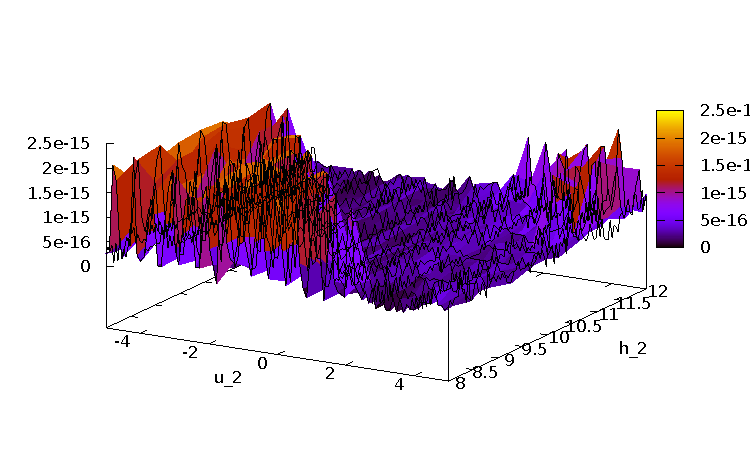
\includegraphics[scale=\zoomfactor]{{{equidist_3_alles_default_ausser_p1_10_-1/10.0_10.0_10.0_0.0_0.0_0.0_10.0_y_10.0_-1.0_x_0.0f00}}}
  % }
  % \subfigure[] {
  %   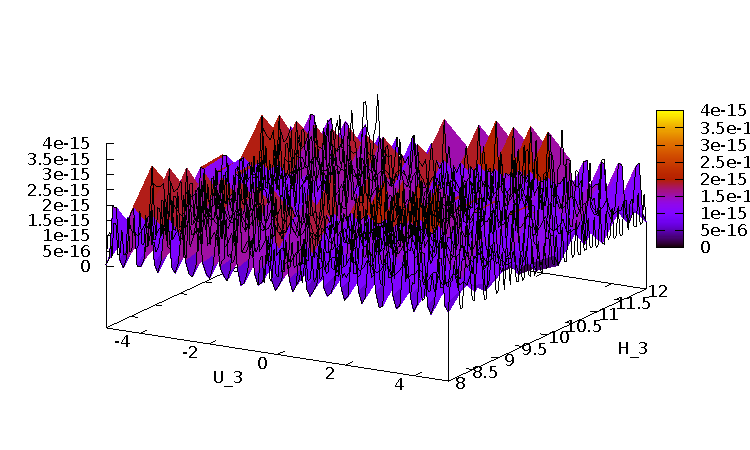
\includegraphics[scale=\zoomfactor]{{{equidist_3_alles_default_ausser_p1_10_-1/10.0_10.0_y_0.0_0.0_x_10.0_10.0_10.0_-1.0_0.0_0.0f00}}}
  % }
  %\subfigure[Impulse error for $p_1^R$] {
  %  \begin{tikzpicture}
  %    \node at (0,0) {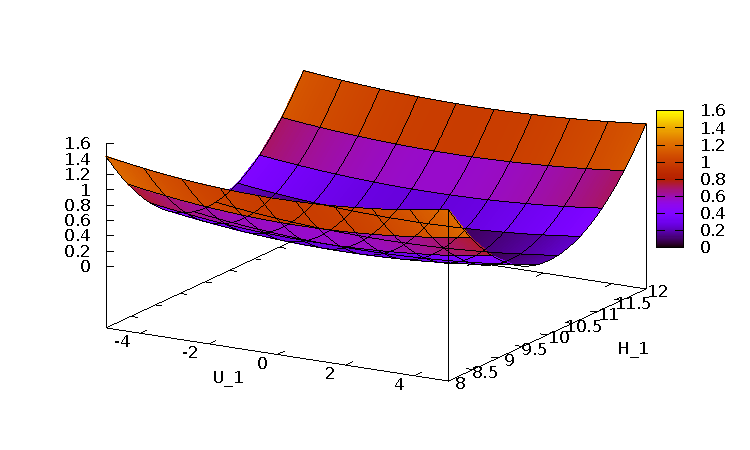
\includegraphics[scale=\zoomfactor]{{{equidist_3_alles_default_ausser_p1_10_-1/y_10.0_10.0_x_0.0_0.0_10.0_10.0_10.0_-1.0_0.0_0.0f01}}}};
  %    \node[align=right, text width=3cm] at (.2,1.33) {\textsf{\tiny{Impulse error}}};
  %    \draw(1.8,1.34) -- +(.4cm,0);
  %  \end{tikzpicture}
  %}
  % \subfigure[] {
  %   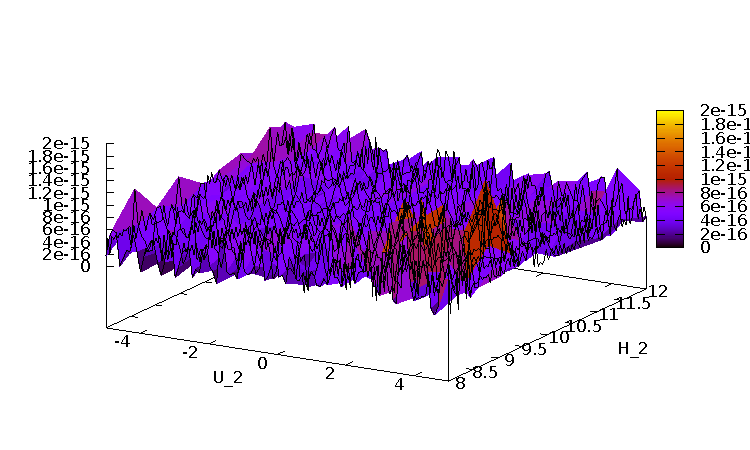
\includegraphics[scale=\zoomfactor]{{{equidist_3_alles_default_ausser_p1_10_-1/10.0_y_10.0_0.0_x_0.0_10.0_10.0_10.0_-1.0_0.0_0.0f00}}}
  % }
  %\subfigure[Impulse error for $p_2^R$] {
  %  \begin{tikzpicture}
  %    \node at (0,0) {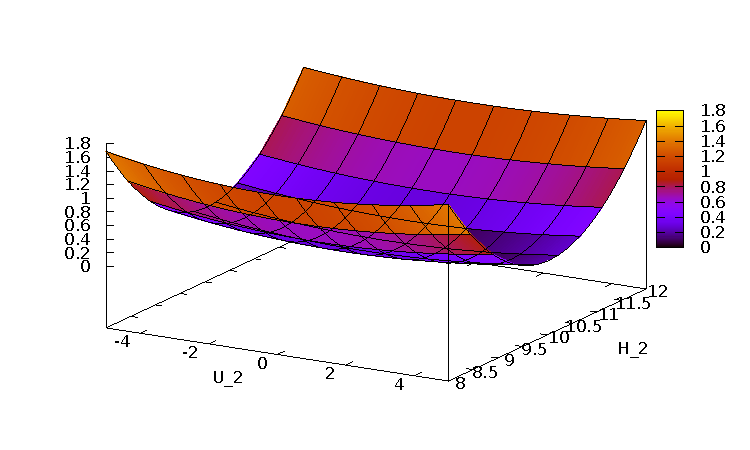
\includegraphics[scale=\zoomfactor]{{{equidist_3_alles_default_ausser_p1_10_-1/10.0_y_10.0_0.0_x_0.0_10.0_10.0_10.0_-1.0_0.0_0.0f01}}}};
  %    \node[align=right, text width=3cm] at (.2,1.33) {\textsf{\tiny{Impulse error}}};
  %    \draw(1.8,1.34) -- +(.4cm,0);
  %  \end{tikzpicture}
  %}
  %\subfigure[Impulse error for $p_3^R$] {
  %  \begin{tikzpicture}
  %    \node at (0,0) {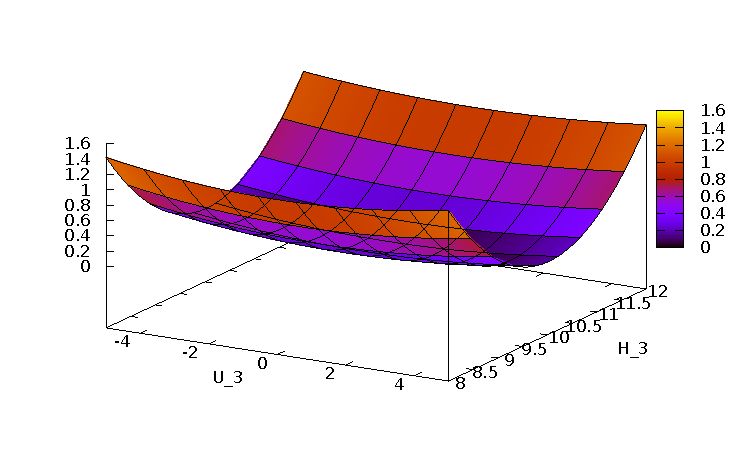
\includegraphics[scale=\zoomfactor]{{{equidist_3_alles_default_ausser_p1_10_-1/10.0_10.0_y_0.0_0.0_x_10.0_10.0_10.0_-1.0_0.0_0.0f01}}}};
  %    \node[align=right, text width=3cm] at (.2,1.33) {\textsf{\tiny{Impulse error}}};
  %    \draw(1.8,1.34) -- +(.4cm,0);
  %  \end{tikzpicture}
  %}
  % \subfigure[] {
  %   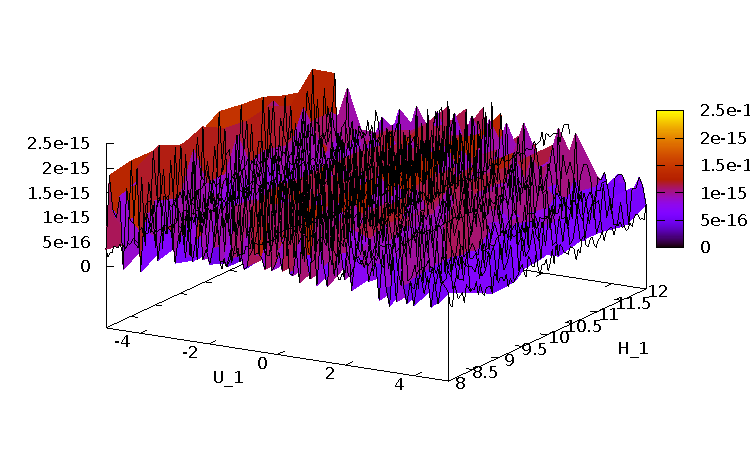
\includegraphics[scale=\zoomfactor]{{{equidist_3_alles_default_ausser_p1_10_-1/y_10.0_10.0_x_0.0_0.0_10.0_10.0_10.0_-1.0_0.0_0.0f00}}}
  % }
\caption{Impulse errors for three equidistant support points at $\{0,\frac{1}{2},1\}$. The point $p_1^L=(10,-1)^T$, all other points are $(10,0)^T$.}
\label{fig:equidist_3_alles_default_ausser_p1_10_-1}
\end{figure}

%%% Local Variables:
%%% TeX-master: "../results.tex"
%%% End:
